\chapter{Learning}
\label{chapter:learning}

This chapter covers the learning part of this dissertation including data collecting, dataset preprocessing, and the models' structures and optimizations.

\section{Problem Introduction}

When anticipating the next action of the user, the object that the user is grasping can provide crucial information about the user's intention. Although an object detection algorithm may be helpful they can suffer from occlusion problems. Therefore, the following models attempt to solve this problem by taking an image of the user grasping a certain object and classifying which object is being grasped using the geometry of the hand.

To obtain a model that would be able to achieve the previous objective two experiments were made. In the first experiment, some types of models were tested with a smaller dataset containing only 300 images per object and 3 objects with the aim of knowing if they would be worth using and optimizing in a more complex problem. In the second experiment, a bigger dataset with 3000 images per object and 4 objects was used to train and optimize the models.

\begin{figure}[H]%[!ht]
    \centering
    \begin{tikzpicture}[>=latex']
    \tikzset{block/.style= {draw, rectangle, align=center,minimum width=3cm,minimum height=1cm},
    rblock/.style={draw, shape=rectangle,rounded corners=1.5em,align=center,minimum width=2cm,minimum height=1cm},
    input/.style={ % requires library shapes.geometric
    draw,
    trapezium,
    trapezium left angle=60,
    trapezium right angle=120,
    minimum width=2cm,
    align=center,
    minimum height=1cm
    },
    }
    
    
    \node [rblock] (camera) {Camera\\Image};
    \node [block, right =3cm of camera] (hands_keypoints) {Mediapipe\\Hands\\Model};
    \node [block, right =3cm of hands_keypoints] (body_keypoints) {Mediapipe\\Full Body\\Model};
    \node [block, below =2cm of body_keypoints] (normalization) {Points\\Normalization};
    \node [block, left =3cm of normalization] (model) {Model\\Prediction};
    \node [rblock, left =3cm of model] (output) {Predicted\\Object};

    %% paths
    \path[draw,->, text width=3cm, align=center]
                (camera) edge (hands_keypoints)
                (camera) edge[bend right] (body_keypoints)
                (hands_keypoints) edge node[above] {{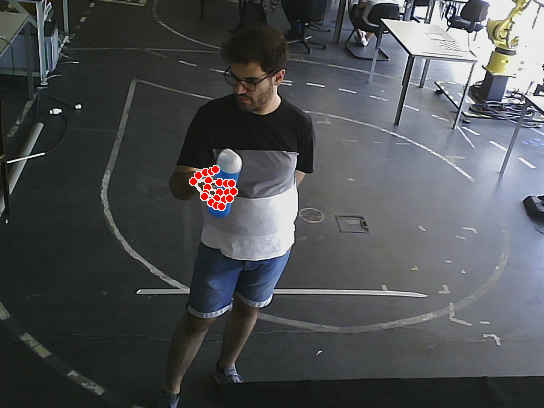
\includegraphics[width=.9\textwidth]{figs/dataset_preprocessing2_1.png}}} (body_keypoints)
                (body_keypoints) edge node[right] {right hand keypoints} (normalization) 
                (normalization) edge node[above] {normalized right hand keypoints} (model)
                (model) edge (output)
                ;

    \if{0}
    \node [rblock] (camera) {Camera\\Image};
    \node [block, right =0.5cm of camera] (hands_keypoints) {Mediapipe\\Hands\\Model};
    \node [block, right =0.5cm of hands_keypoints] (body_keypoints) {Mediapipe\\Full Body\\Model};
    \node [block, right =0.5cm of body_keypoints] (normalization) {Points\\Normalization};
    \node [block, right =0.5cm of normalization] (model) {Model\\Prediction};
    \node [rblock, right =0.5cm of model] (output) {Predicted\\Object};

    %% paths
    \path[draw,->, text width=1.7cm, align=center]
                (camera) edge (hands_keypoints)
                (camera) edge[bend right] (body_keypoints)
                (hands_keypoints) edge (body_keypoints)
                (body_keypoints) edge (normalization) 
                (normalization) edge (model)
                (model) edge (output)
                ;
    \fi
    
\end{tikzpicture}
    \caption{Machine Learning Pipeline}
    \label{fig:ml_pipeline}
\end{figure}


\section{Data Collecting}

The first step to train a supervised machine learning model is to find a dataset. However, given that this problem is very specific the datasets had to be manually collected. For this purpose, 2 datasets were collected with both consisting of a set of videos where one person would be moving and rotating a certain object. These videos were recorded at 10 frames per second to avoid consecutive frames having similar hand poses.

\begin{figure}[H]
\centerline{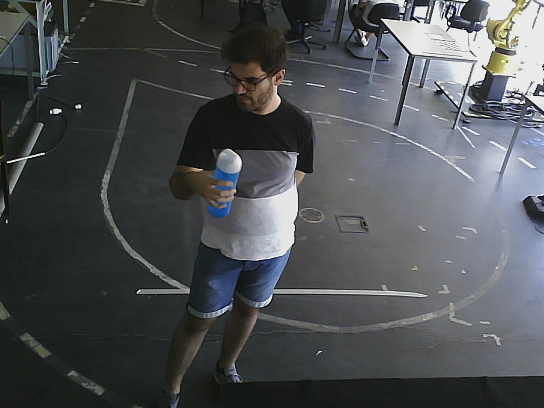
\includegraphics[width=0.49\textwidth]{figs/dataset_preprocessing1_1.png} 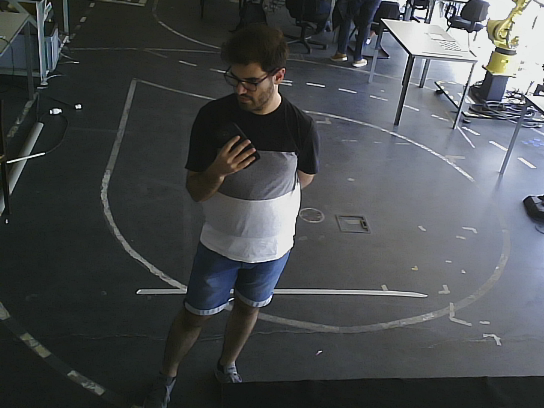
\includegraphics[width=0.49\textwidth]{figs/dataset_preprocessing1_2.png}}
\caption[Dataset Examples]{Dataset Examples}
\label{fig:dataset_examples}
\end{figure}

In the first dataset, 3 different objects were used (see Fig: x), and for each one, 1 person was recorded for 30 seconds resulting in 300 images per object. In the second dataset, 4 objects were used (see Fig: x), and 3 people were recorded in 4 different 25-second videos for each object resulting in 1000 frames for each person and object making it 3000 frames for each object. Recording more than one video for each combination of person and object allowed each person to grasp the object slightly differently each time in order to obtain a more diverse dataset.

\textcolor{red}{image with objects}

\section{Dataset Preprocessing}

After having a dataset, the data had to be processed so that it would have a fitting structure to be used in the model training and testing. The images from the videos were processed using the Mediapipe hands model resulting in 21 points for each hand detected. The images were also processed by the full-body model also provided by Mediapipe so that it is possible to identify the right hand.

\begin{figure}[H]
\centerline{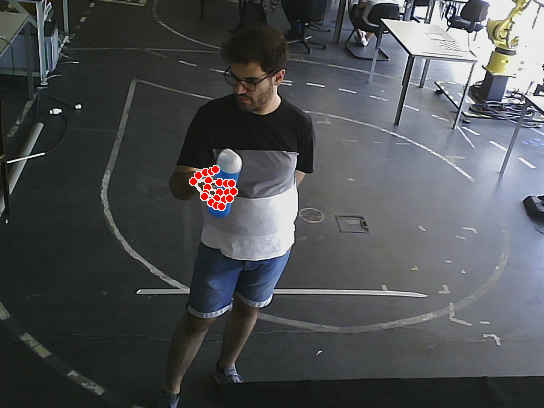
\includegraphics[width=0.49\textwidth]{figs/dataset_preprocessing2_1.png} 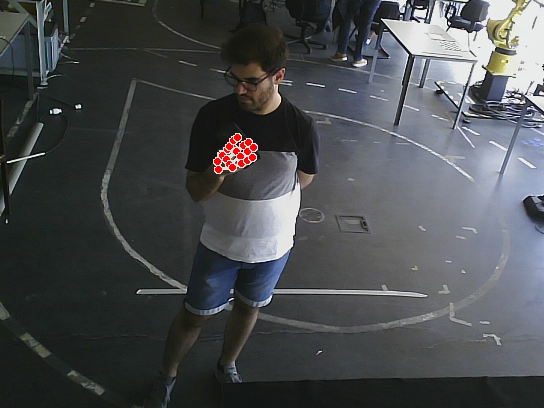
\includegraphics[width=0.49\textwidth]{figs/dataset_preprocessing2_2.png}}
\caption[Dataset Examples]{Dataset Examples}
\label{fig:dataset_examples}
\end{figure}

These points are then subject to further processing and normalization so that the location of the hand in the image and the distance between the hand and the camera have a lesser impact. The centroid is calculated and the points are translated so that they are centered in the (0.5, 0.5, 0.5) point, the points are then scaled up as much as possible while keeping every coordinate of every point between 0 and 1.

\begin{figure}[H]
\centerline{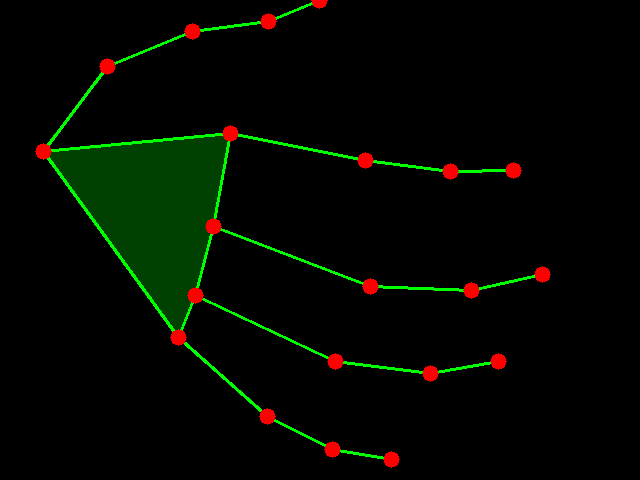
\includegraphics[width=0.49\textwidth]{figs/dataset_preprocessing3_1.png} 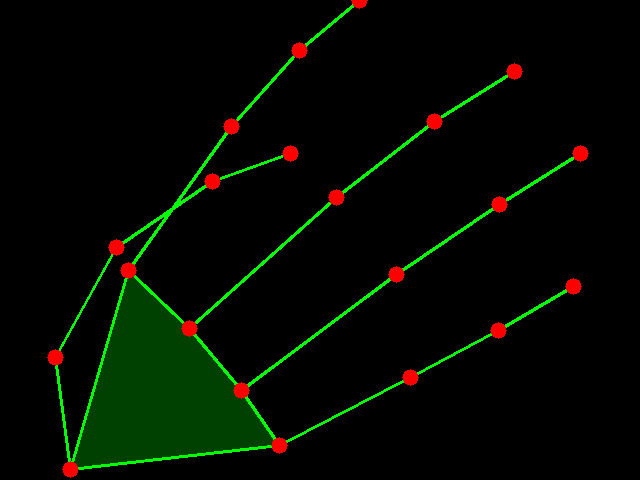
\includegraphics[width=0.49\textwidth]{figs/dataset_preprocessing3_2.png}}
\caption[Dataset Examples]{Dataset Examples}
\label{fig:dataset_examples}
\end{figure}

\section{Data Splitting}

In order to train the model, the dataset was split into 3 sets: the train set (60\%), the validation set (20\%), and the test set (20\%). The random variables in the data shuffling and splitting were also fixed so that the test set is always the same, and therefore, its data is never used to train or validate the model, even in different trains. During hyperparameter optimization, the different combinations are tested using 4-fold cross-validation, which means that the model is trained 4 times, and therefore every sample of data in the initial training and validation set was used both for training and validation. Additionally, early stopping was set up so that the model would stop after 200 epochs without a better validation loss.

\section{Models}

\subsection{Convolutional Neural Network}

After all the processing, each sample provided to the model is made of the 21 points that represent the right hand. Given that points are related to each other, a one-dimensional convolutional neural network was used to take advantage of this characteristic. Therefore, the CNN is responsible for taking the 21 3D points and classifying the object that is being grasped.

\subsubsection{Initial Results}

Initially, a simple CNN was tested and manually optimized with the first dataset resulting in the following results:

\begin{minipage}{0.35\textwidth}
    \captionof{table}{CNN Results in the First Dataset}
    \label{table:cnn_dataset1_results}
    \centering
    \begin{tabular}{ |p{3.4cm}|p{1.1cm}| }
    \hline
    Metric & Value \\
    \hline
    Training Accuracy & 0.9813 \\
    \hline
    Validation Accuracy & 0.9775 \\
    \hline
    Test Accuracy & 0.9551 \\
    \hline
    Training Loss & 0.0493 \\
    \hline
    Validation Loss & 0.0794 \\
    \hline
    Test Loss & 0.1600 \\
    \hline
    Precision & 0.9583 \\
    \hline
    Recall & 0.9551 \\
    \hline
    F1-Score & 0.9549 \\
    \hline
    \end{tabular}
\end{minipage}%
\begin{minipage}{0.65\textwidth}
    \centering
    \includesvg[width=\textwidth]{figs/cnn_dataset1_conf_matrix.svg}
    %\def\svgwidth{\columnwidth}
    %\input{figs/cnn_dataset1_conf_matrix.pdf_tex}
    \captionof{figure}[CNN Confusion Matrix in the First Dataset]{CNN Confusion Matrix in the First Dataset}
    \label{fig:cnn_confusion_matrix}
\end{minipage}

\kern 0.1cm

Even with a relatively small dataset, this CNN shows positive results with accuracies over 95\%, so it was decided that this model should be tested in the second dataset.

\subsubsection{Final Model Architecture}

When training a model with the initial architecture in the second dataset, the results were considerably lower than those achieved with the first dataset. Given that not only the dataset was bigger, but there was also one more class, it was decided that the model should have a more complex architecture, and with manual optimizations a new architecture was created which had better results. The new model can be seen on Fig.~\ref{fig:cnn_architecture} and it is made of 2 convolutional layers followed by 3 dense layers, with the third being the output layer. Between the convolutional and the dense layers and between both dense layers there is also a dropout layer so as to help with overfitting.

\begin{figure}[H]%[!ht]
    \centering
    \begin{tikzpicture}[>=latex']
    \tikzset{block/.style= {draw, rectangle, align=center,minimum height=2.5cm, scale=1.2},
    rblock/.style={draw, shape=rectangle,rounded corners=1.5em,align=center,minimum width=2cm,minimum height=1cm},
    input/.style={ % requires library shapes.geometric
    draw,
    trapezium,
    trapezium left angle=60,
    trapezium right angle=120,
    minimum width=2cm,
    align=center,
    minimum height=1cm
    },
    }
    
    \node [block] (inputlayer) {\rotatebox{90}{InputLayer}};
    \node [block, right=0.5cm of inputlayer] (conv1d_1) {\rotatebox{90}{Conv1D}};
    \node [block, right=0.5cm of conv1d_1] (conv1d_2) {\rotatebox{90}{Conv1D}};
    \node [block, right=0.5cm of conv1d_2] (flatten) {\rotatebox{90}{Flatten}};
    \node [block, right=0.5cm of flatten] (dropout_1) {\rotatebox{90}{Dropout}};
    \node [block, right=0.5cm of dropout_1] (dense_1) {\rotatebox{90}{Dense}};
    \node [block, right=0.5cm of dense_1] (dropout_2) {\rotatebox{90}{Dropout}};
    \node [block, right=0.5cm of dropout_2] (dense_2) {\rotatebox{90}{Dense}};
    \node [block, right=0.5cm of dense_2] (dense_3) {\rotatebox{90}{Dense}};

    %% paths
    \path[draw,->, text width=3cm, align=center]
                (inputlayer) edge (conv1d_1)
                (conv1d_1) edge (conv1d_2)
                (conv1d_2) edge (flatten)
                (flatten) edge (dropout_1)
                (dropout_1) edge (dense_1)
                (dense_1) edge (dropout_2)
                (dropout_2) edge (dense_2)
                (dense_2) edge (dense_3)
                ;
    
\end{tikzpicture}
    \caption[CNN Architecture]{CNN Model Architecture}
    \label{fig:cnn_architecture}
\end{figure}

%\begin{figure}[H]
%\centerline{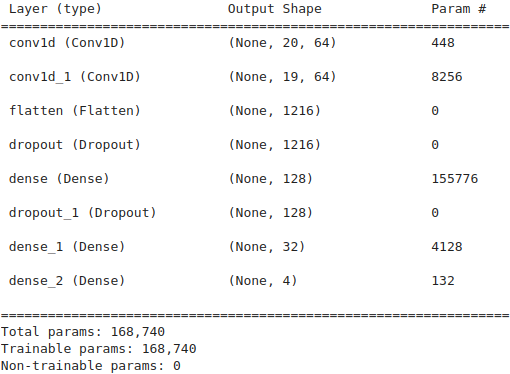
\includegraphics[height=3.4in]{figs/cnn_architecture.png}}
%\caption[CNN Architecture]{CNN Model Architecture}
%\label{fig:cnn_architecture}
%\end{figure}

\subsubsection{Hyperparameter Optimization}

In this model, 3 common hyperparameters in CNNs were optimized to obtain better results. These were the initial learning rate for the model training, the kernel size used by the convolutional layers and the dropout rate. Additionally, the number of convolutional layers was also tested given that, according to manual testing, it also affected the model results without changing the number of trainable parameters. The values tested for each hyperparameter can be seen on Table \ref{table:cnn_hyperparameters}.

\begin{table}[H]
\caption{Tested Hyperparameter Values}
\label{table:cnn_hyperparameters}
\centering
\begin{tabular}{|l|l|}
\hline
Hyperparameter & Tested Values \\
\hline
Learning Rate & 0.01, 0.001, 0.0001 \\
\hline
Number of Convolutional Layers & 1, 2, 3 \\
\hline
Kernel Size & 2, 3 \\
\hline
Dropout Rate & 0.0, 0.1, 0.2, 0.3, 0.4, 0.5 \\
\hline
\end{tabular}
\end{table}

In order to choose the best combination of these hyperparameters, all combinations were tested using 4-fold cross validation, which means that the model was trained 4 times, and every sample of data was used both for training and validation. It is important to note that the process to obtain these hyperparameters did not include the data from the test set. Then the average result of each combination was obtained with the combination in Table \ref{table:cnn_best_hyperparameters} having the lowest average loss with 0.2100 and an average accuracy of 94.20\%.

\begin{table}[H]
\captionof{table}{CNN Best Hyperparameters}
\label{table:cnn_best_hyperparameters}
\centering
\begin{tabular}{|l|l|}
\hline
Hyperparameter & Value \\
\hline
Learning Rate & 0.001 \\
\hline
Dropout & 0.5 \\
\hline
Kernel Size & 3 \\
\hline
Number of Convolutional Layers & 2 \\
\hline
\end{tabular}
\end{table}

\subsubsection{Final Results}

With the final architecture defined as well as the model hyperparameters, the final model was trained with the data of the second dataset. The Fig.~\ref{fig:cnn_loss} and Fig.~\ref{fig:cnn_acc} show the evolution of the training and validation loss and accuracy respectively during the training. According to the figures, the best validation loss occurred slightly after the 400th epoch with training stopping 200 epochs later.

% using pretex=\scriptsize reduces all fonts size
\begin{figure}[H]
\centerline{\includesvg[width=\textwidth, pretex=\scriptsize]{figs/cnn_loss_comparison.svg}}
\caption[CNN training and validation loss evolution during training]{CNN training and validation loss evolution during training}
\label{fig:cnn_loss}
\end{figure}

\begin{figure}[H]
\centerline{\includesvg[width=\textwidth, pretex=\scriptsize]{figs/cnn_acc_comparison.svg}}
\caption[CNN training and validation accuracy evolution during training]{CNN training and validation accuracy evolution during training}
\label{fig:cnn_acc}
\end{figure}

With training completed, the metrics in the Table \ref{table:cnn_dataset2_results} were obtained. Given that the validation and test accuracies are close to each other we can conclude that the model managed to generalize its knowledge from the training data to classify data it has never seen before. Additionally, the confusion matrix in the Fig.~\ref{fig:cnn_confusion_matrix} shows that the screwdriver was the object that the model managed to predict more accurately. This can be due to the fact that the hand geometry that allows a person to grasp a screwdriver intuitively is more restrict.

\begin{minipage}{0.35\textwidth}
    \captionof{table}{CNN Results in the Second Dataset}
    \label{table:cnn_dataset2_results}
    \centering
    \begin{tabular}{ |p{3.4cm}|p{1.1cm}| }
    \hline
    Metric & Value \\
    \hline
    Training Accuracy & 0.9601 \\
    \hline
    Validation Accuracy & 0.9442 \\
    \hline
    Test Accuracy & 0.9400 \\
    \hline
    Training Loss & 0.1191 \\
    \hline
    Validation Loss & 0.2171 \\
    \hline
    Test Loss & 0.2291 \\
    \hline
    Precision & 0.9403 \\
    \hline
    Recall & 0.9400 \\
    \hline
    F1-Score & 0.9400 \\
    \hline
    \end{tabular}
\end{minipage}%
\begin{minipage}{0.65\textwidth}
    \centering
    \includesvg[width=\textwidth]{figs/cnn_conf_matrix.svg}
    \captionof{figure}[CNN confusion matrix]{CNN confusion matrix}
    \label{fig:cnn_confusion_matrix}
\end{minipage}

\subsection{Transformer Neural Network}

As said in Subsection \ref{subsection:transformer_neural_networks}, Transformer Neural Networks shine at capturing long-range dependencies and relationships. Therefore, considering the fact that the points obtained from Mediapipe have a specific order, we can take advantage of this ability to process structured data and effectively capture dependencies and patterns.

\subsubsection{Initial Results}

Initially, a Transformer architecture from \textcolor{red}{link} was tested and manually optimized with the first dataset resulting in the following results:

\begin{minipage}{0.35\textwidth}
    \captionof{table}{Tranformer Results in the First Dataset}
    \label{table:transformer_dataset1_results}
    \centering
    \begin{tabular}{ |p{3.4cm}|p{1.1cm}| }
    \hline
    Metric & Value \\
    \hline
    Training Accuracy & 0.8820 \\
    \hline
    Validation Accuracy & 0.8989 \\
    \hline
    Test Accuracy & 0.8820 \\
    \hline
    Training Loss & 0.2794 \\
    \hline
    Validation Loss & 0.2926 \\
    \hline
    Test Loss & 0.3600 \\
    \hline
    Precision & 0.9081 \\
    \hline
    Recall & 0.8820 \\
    \hline
    F1-Score & 0.8835 \\
    \hline
    \end{tabular}
\end{minipage}%
\begin{minipage}{0.65\textwidth}
    \centering
    \includesvg[width=\textwidth]{figs/transformer_dataset1_conf_matrix.svg}
    %\def\svgwidth{\columnwidth}
    %\input{figs/cnn_dataset1_conf_matrix.pdf_tex}
    \captionof{figure}[Transformer Confusion Matrix in the First Dataset]{Transformer Confusion Matrix in the First Dataset}
    \label{fig:transformer_confusion_matrix}
\end{minipage}

\kern 0.1cm

Even with a relatively small dataset, this Transformer shows positive results with accuracies over 88\%. However, when considering the accuracies in each class, we can see that it has greater difficulty in distinguishing between two similar objects. Despite this, it was decided that this model should be tested in the second dataset.

\subsubsection{Model Architecture}

\subsubsection{Hyperparameter Optimization}

\begin{table}[H]
\caption{Tested Hyperparameter Values}
\label{table:transformer_hyperparameters}
\centering
\begin{tabular}{|l|l|}
\hline
Hyperparameter & Tested Values\\
\hline
Learning Rate & 0.01, 0.001, 0.0001\\
\hline
Dropout Rate & 0.0, 0.1, 0.2, 0.3, 0.4, 0.5\\
\hline
MLP Dropout Rate & 0.0, 0.1, 0.2, 0.3, 0.4, 0.5\\
\hline
\end{tabular}
\end{table}

In order to choose the best combination of these hyperparameters, all combinations were
tested using 4-fold cross-validation, and the combination with the smallest average validation loss was chosen. This combination can be seen in Table \ref{table:transformer_best_hyperparameters}
having an average loss of 0.2594 and an average accuracy of 92.24\%.

\begin{table}[H]
\captionof{table}{Transformer Best Hyperparameters}
\label{table:transformer_best_hyperparameters}
\centering
\begin{tabular}{|l|l|}
\hline
Hyperparameter & Value \\
\hline
Learning Rate & 0.0001 \\
\hline
Dropout Rate & 0.5 \\
\hline
MLP Dropout Rate & 0.1 \\
\hline
\end{tabular}
\end{table}

\subsubsection{Final Results}

% using pretex=\scriptsize reduces all fonts size
\begin{figure}[H]
\centerline{\includesvg[width=\textwidth, pretex=\scriptsize]{figs/transformer_loss_comparison.svg}}
\caption[Transformer training and validation loss evolution during training]{Transformer training and validation loss evolution during training}
\label{fig:transformer_loss}
\end{figure}

\begin{figure}[H]
\centerline{\includesvg[width=\textwidth, pretex=\scriptsize]{figs/transformer_acc_comparison.svg}}
\caption[Transformer training and validation accuracy evolution during training]{Transformer training and validation accuracy evolution during training}
\label{fig:transformer_acc}
\end{figure}

\begin{minipage}{0.35\textwidth}
    \captionof{table}{Transformer Results in the Second Dataset}
    \label{table:transformer_dataset2_results}
    \centering
    \begin{tabular}{ |p{3.4cm}|p{1.1cm}| }
    \hline
    Metric & Value\\
    \hline
    Training Accuracy &  0.9414\\
    \hline
    Validation Accuracy & 0.9263\\
    \hline
    Test Accuracy & 0.9244\\
    \hline
    Training Loss & 0.1675\\
    \hline
    Validation Loss & 0.2830\\
    \hline
    Test Loss & 0.2404\\
    \hline
    Precision & 0.9244\\
    \hline
    Recall & 0.9244\\
    \hline
    F1-Score & 0.9243\\
    \hline
    \end{tabular}
\end{minipage}%
\begin{minipage}{0.65\textwidth}
    \centering
    \includesvg[width=\textwidth]{figs/transformer_conf_matrix.svg}
    \captionof{figure}[Transformer confusion matrix]{Transformer confusion matrix}
    \label{fig:transformer_confusion_matrix}
\end{minipage}

\section{Models Comparison}

\begin{table}[H]
\caption{Results with data from one user}
\label{table:results_one_user}
\centering
\begin{tabular}{|l|l|l|l|l|l|l|l|l|} 
\hline
& \multicolumn{4}{|l|}{Loss} & \multicolumn{4}{|l|}{Accuracy} \\
\hline
Model & P1 & P2 & P3 & AVG & P1 & P2 & P3 & AVG \\
\hline
CNN & 0.1897 & 0.3179 & 0.2758 & 0.2611 & 0.9673 & 0.9243 & 0.9378 & 0.9431 \\
\hline
Transformer & \_ & \_ & \_ & \_ & \_ & \_ & \_ & \_ \\
\hline
\end{tabular}
\end{table}

\begin{table}[H]
\caption{Results with a different test user in relation to training}
\label{table:results_2vs1_user}
\centering
\begin{tabular}{|l|l|l|l|l|l|l|l|l|} 
\hline
& \multicolumn{4}{|l|}{Loss} & \multicolumn{4}{|l|}{Accuracy} \\
\hline
Model & P1 & P2 & P3 & AVG & P1 & P2 & P3 & AVG \\
\hline
CNN & 0.6625 & 2.1951 & 1.8477 & 1.5684 & 0.7958 & 0.5970 & 0.5417 & 0.6448 \\
\hline
Transformer & \_ & \_ & \_ & \_ & \_ & \_ & \_ & \_ \\
\hline
\end{tabular}
\end{table}

\section{\textcolor{red}{Integration with Previous Work}}